\documentclass[UTF8]{ctexart}
\usepackage{amsmath}
\usepackage{amssymb}
\usepackage{background}
\usepackage{booktabs}
\usepackage{caption,subcaption}
\usepackage{enumitem}
\usepackage{fancyhdr}
\usepackage{float}
\usepackage{fontspec}
%\usepackage{fourier}
\usepackage{geometry}
\usepackage{makecell}
\usepackage{tcolorbox}
\tcbuselibrary{breakable, raster}
\usepackage{tikz}
\usetikzlibrary{arrows.meta}
\usepackage{xcolor}

\geometry{a5paper, top=0.1cm, left=1cm, right=1cm, bottom=1cm, footskip=0.6cm, marginparsep=0.1cm}

\setCJKmainfont[BoldFont={汉仪文黑-85W},ItalicFont={方正苏新诗柳楷简体}]{汉仪文黑-55W}
\setfontfamily\Issue{Century Schoolbook}
\setfontfamily\Genshin{Genshin Teyvat Lingua Franca}
\newCJKfontfamily\TitleFont{思源宋体 CN Heavy}
\newfontfamily\timesnewroman{Times New Roman}
\captionsetup{font=small, labelfont=bf}
\setlist[itemize]{itemsep=0pt, parsep=0pt}
\pagestyle{fancy}
\fancyhf{}
\cfoot{\ttfamily\footnotesize{-\ \thepage\ -}}
%\reversemarginpar

%\CTEXsetup[format = {\centering\bfseries\large}, beforeskip = 3pt, afterskip = 3pt]{section}
\CTEXsetup[format = {\color{cyan!50!black}\bfseries\large}]{subsection}

\newcommand\col[1]{\textcolor{darkcyan}{#1}}
\newcommand\AND{\  \textrm{AND}\ }
\newcommand\OR{\  \textrm{OR}\ }
\newcommand\IF{\quad\textrm{IF}\quad}
\newcommand\THEN{\quad\textrm{THEN}\quad}
\newcommand\CF{{C\hspace{-0.2em}F}}
\newcommand\relation[2]{\langle #1 , #2 \rangle}

\newtcolorbox{process}[1]{colback=cyan!10, colframe=cyan!50!black, boxrule=0.5pt, title={#1}, breakable}

\colorlet{darkcyan}{cyan!50!black}
\newcommand\Black[1]{\textcolor[gray]{0.3}{#1}}
\newcommand\Brown[1]{\textcolor[HTML]{998A4E}{#1}}
\newcommand\Emph[1]{\colorbox{green!10}{\textcolor{green!30!black}{#1}}}
\newcommand\Concept[1]{\textcolor{cyan!70!black}{#1}}
\newcommand\Notes[1]{\textcolor{yellow!50!black}{\small #1}}
\newcommand\Example[1]{\textcolor{cyan!70!black}{\small #1}}
\newcommand\means[1]{\textcolor{cyan!70!black}{#1}}


\newcommand\C{\mathrm{C}}
\newcommand\e{\mathrm{e}}
\renewcommand\d{\mathrm{d}}
\newcommand\Cov{\mathrm{Cov}}
\renewcommand\pi{\text{\timesnewroman π}}

\newcommand\IssueNumber{40}
\newcommand\Date{2024-11-4}
%\newcommand\Contributer{@金光日}
\newcommand\Subject{人工智能}
%\newcommand\Source{2022 考研 408 第 5 题}


\begin{document}
\backgroundsetup{contents=
\includegraphics{上半示例.png}, center, scale=1, angle=0, opacity=1}
\BgThispage
\begin{center}
%{\scriptsize\Issue \textcolor[HTML]{C8BA83}{\Genshin WEEKLY TIPS}}
\phantom{...}

{\Large\textcolor{brown!40!white}{\makebox[10cm][s]{\Genshin WEEKLY KNOWLEDGE TIPS}}}

\vspace{-2em}

{\Huge\bfseries\TitleFont \Black{知\ 识\ 小\ 料}}


\vspace{-0.1cm}
{\footnotesize \Brown{「电计 2203 班」周常规知识整理共享}}
\end{center}

\vspace{-0.5cm}


\begin{figure}[H]
\hspace{1cm}
\begin{minipage}[t]{0.3\textwidth}
\centering
    \Brown{\Genshin ISSUE}

    \vspace{-0.6cm}
    \Huge \Issue\slshape\bfseries\Black{\IssueNumber}
\end{minipage}
\hfill
\begin{minipage}[t]{0.35\textwidth}
\small
\centering
    \Brown{日期:\Date} \\
%\vspace{-0.1cm}
%    \Brown{贡献者:\Contributer} \\
\vspace{-0.1cm}
    \Brown{学科:\Subject} \\
%\vspace{-0.1cm}
%    \Brown{来源:\Source}
\end{minipage}
\hspace{0.8cm}
\end{figure}

{\color{cyan!50!black}
本文档用于对《人工智能》课程作出简明复习。}

\section{人工智能概述}
人工智能的英语为 Artificial Intelligence,日语为「$\stackrel{\text{じんこうちのう}}{\text{人工知能}}$」。

狭义:人工的方法在机器上实现的智能;广义:人类智能行为规律、智能理论方面的研究。

三次低谷:
\begin{itemize}[itemsep=0pt,parsep=0pt]
  \item 第一次低谷:1973年英国发表James Lighthill 报告;
  \item 第二次低谷:日本智能(第五代)计算机研制失败;
  \item 第三次低谷:知识词典日趋势微、网络百科兴起
\end{itemize}

三个发展阶段:弱人工智能、强人工智能、超人工智能。

三个主流方法:符号主义、数据驱动、探索与利用。
\begin{itemize}[itemsep=0pt,parsep=0pt]
  \item 符号主义人工智能为核心的逻辑推理;
  \item 数据驱动为核心的机器学习;
  \item 探索与利用为核心的强化学习。
\end{itemize}

\section{知识与谓词逻辑}
知识的特性:相对正确性、不确定性、可表示性与可利用性。其中,不确定性由随机性、模糊性、经验性、不完全性引起。

\Emph{神经网络}属于知识的一种表示形式。

事实与规则的区别。事实:「$p$ 是 $q$」;规则:「若 $p$ 则 $q$」。

\subsection{一阶谓词逻辑}
涉及到以下概念:
\begin{itemize}[itemsep=0pt,parsep=0pt]
  \item 命题、命题逻辑;谓词、个体;
  \item 连接词 5 个(依次为 $\neg\ \wedge\ \vee\ \to\ \leftrightarrow$)、量词 2 个、谓词公式;
  \item 辖域、约束变元、自由变元、等价式
  \item 解释:永真、永假、可满足
\end{itemize}

常见的推理规则:
\begin{itemize}[itemsep=0pt,parsep=0pt]
  \item 假言推理:$P,\ P\to Q \implies Q$
  \item 拒取式推理:$\neg Q, \ P\to Q \implies \neg P$
  \item 假言三段论:$P\to Q,\ Q\to R \implies P\to R$
  \item 全称固化、存在固化、反证法。
\end{itemize}

\backgroundsetup{contents=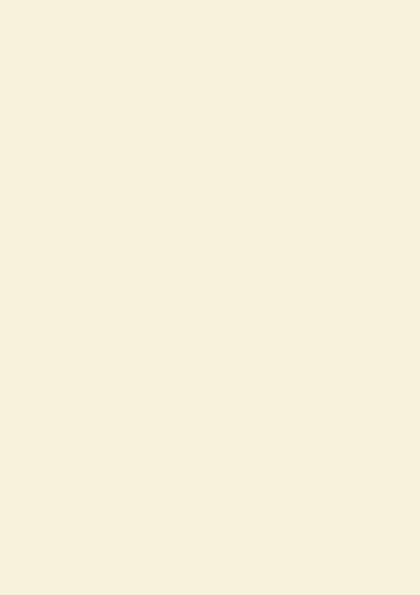
\includegraphics{空白示例.png}, center, scale=1, angle=0, opacity=1}
\BgThispage
\subsection{产生式与框架}
四种产生式表示法\footnote{object:对象;attribute:属性;value:值;relationship:关系,$x$:置信度。}:
\begin{itemize}[itemsep=0pt,parsep=0pt]
  \item 确定性规则的知识:$\mathrm{IF}\ P\ \mathrm{THEN}\ Q$
  \item 不确定性规则的知识:$\mathrm{IF}\ P\ \mathrm{THEN}\ Q\quad (x)$
  \item 确定性事实的知识:$(obj, attr, val)$ 或者 $(rel, obj_1, obj_2)$
  \item 不确定性事实的知识:$(obj, attr, val, x)$ 或者 $(rel, obj_1, obj_2, x)$
\end{itemize}

产生式的形式表示:BNF「巴科斯范式」。

产生式系统例子:动物识别系统。

框架、槽、侧面,相当于类与对象的关系。

知识图谱是互联网环境下的知识表示方法,通用表示形式是三元组。举例如维基百科、百度百科等。

\section{确定性推理(离散数学·数理逻辑)}
推理方式分类:
\begin{itemize}[itemsep=0pt,parsep=0pt]
    \item 演绎推理:一般$\to$个别;
    \item 归纳推理:个别$\to$一般;
    \item 默认推理:假设某些条件默认成立的推理。
\end{itemize}
还有的按照确定性/不确定性推理、单调/非单调推理、启发式/非启发式推理。默认推理为非单调推理。

推理方向:正向、逆向、混合、双向推理。

多种匹配成功,则采用冲突消解策略。

自然演绎推理,包含规则:$P$ 规则(给定前提)、$T$ 规则(产生的结论作前提)、假言推理、拒取式推理等。

\subsection{谓词公式化子句集}
谓词公式化子句集一般包含以下九个步骤:
\begin{enumerate}[itemsep=0pt,parsep=0pt]
  \item 消去条件、双条件符号($\to\ \leftrightarrow$);
  \item 把 $\neg$ 移到紧靠字母的位置;
  \item 存在量词标准化;
  \item 消去存在量词:$(\forall x)(\exists \col{y})P(x,\col{y}) \iff (\forall x)P(x, \col{f(x)})$;
  \item 化为前束范式:前缀+主表达式;
  \item 化为斯科伦范式:$\textbullet \wedge \textbullet \wedge \textbullet$;
  \item 删除全称量词;
  \item 消去 $\wedge$ 并改成集合形式;
  \item 子句变量标准化。
\end{enumerate}

谓词公式不可满足 $\iff$ 子句集不可满足。

\subsection{鲁宾逊归结原理}
只要能归结出\Emph{空子句},则证明子句集不可满足。

应用归结反演求解问题。可能引入 $ANSWER$ 子句参与归结。(需要练习)

\section{不确定性推理}
不确定性的表示与度量:
\begin{itemize}[itemsep=0pt,parsep=0pt]
  \item 知识不确定性的表示——知识的静态强度:$\CF (H,E)$
  \item 证据不确定性的表示——证据的动态强度:$\CF (E)$
\end{itemize}

\subsection{可信度分析:C-F模型}
对于产生式 $\IF E \THEN H (\CF (H,E))$,$\CF(H,E)\in[-1,1]$,正数表示 $E$ 支持 $H$ 为真,负数表示 $E$ 支持 $H$ 为假。

具体包括以下规则:\textcolor{cyan}{(参见「知识小料」·其三十五)}
\begin{itemize}[itemsep=0pt,parsep=0pt]
  \item 合取规则:$\CF(E_1\AND E_2) = \min\{\CF(E_1),\ \CF(E_2)\}$
  \item 析取规则:$\CF(E_1\OR E_2) = \max\{\CF(E_1),\ \CF(E_2)\}$
  \item 传递规则:$\CF(H) = \CF(H,E)\cdot \max\{0,\CF(E)\}$
  \item 合成规则:若有 $\begin{cases}
  \IF E_1 \THEN H\quad  (\CF(H,E_1))\\
  \IF E_2 \THEN H\quad  (\CF(H,E_2))
   \end{cases}$
    ,须先由传递规则算出 $a=\CF_1(H)$、$b=\CF_2(H)$。设 $S=\CF_{12}(H)$,则
      \begin{enumerate}[itemsep=2pt,parsep=0pt]
        \item 当 $a\geqslant 0,b\geqslant 0$ 时,$S = a+b-ab$
        \item 当 $a<0,b<0$ 时,$S = a+b+ab$
        \item 当 $a,b$ 异号时,$S = \dfrac{a+b}{1-\min\{|a|,|b|\}}$
      \end{enumerate}
\end{itemize}

证据理论:概率分配函数、信任函数 $Bel$、似然函数 $Pl$ 等。

\subsection{模糊集}
模糊集,可理解为刨除「确定性」的集合,允许元素对集合的隶属度有一个浮动的值。

假设论域(全集)为 $U=\{a,b,c\}$,则下表 \ref{tab:fuzzy-set} 给出了模糊集与普通集合的一个对照表。
\begin{table}[htb]
  \centering
  \begin{tabular}{|c|c|c|}
    \hline
    & 普通集合 & 模糊集 \\
    \hline
    举例 & $A=\{a,b\}$、$B=\{a,c\}$ & $A=\left\{\frac{0.5}{a},\frac{0.4}{b}\right\}$、$B=\left\{\frac{0.3}{a},\frac{0.6}{c}\right\}$ \\
    \hline
    交集 & $A\cap B=\{a\}$ & \makecell{$A\cap B=\left\{\frac{\min(0.5,0.3)}{a},\frac{\min(0.4,0)}{b},\frac{\min(0,0.6)}{c}\right\} $ \\
    $= \left\{\frac{0.3}{a}\right\}$} \\
    \hline
    并集 & $A\cup B=\{a,b,c\}$ & \makecell{$A\cup B=\left\{\frac{\max(0.5,0.3)}{a},\frac{\max(0.4,0)}{b},\frac{\max(0,0.6)}{c}\right\} $ \\ $= \left\{\frac{0.5}{a}, \frac{0.4}{b}, \frac{0.6}{c}\right\}$} \\
    \hline
    补集 & $\bar{A} = U\backslash A = \{c\}$ & \makecell{$\bar{A} = \left\{\frac{1-0.5}{a},\frac{1-0.4}{b}, \frac{1}{c}\right\}$ \\ $=\left\{\frac{0.5}{a},\frac{0.6}{b},\frac{1}{c}\right\}$} \\
    \hline
    \makecell{笛卡\\尔积} & \makecell{$A\times B = \{\relation{a}{a}, \relation{a}{c}, $ \\ $\relation{b}{a}, \relation{b}{c}\}$} & $\begin{aligned}
        A\times B &= \begin{bmatrix}
                       0.5 \\ 0.4
                     \end{bmatrix}\circ \begin{bmatrix} 0.3 &  0 & 0.6\end{bmatrix} \\
        &= \begin{bmatrix}
             0.3 & 0 & 0.5 \\
             0.3 & 0 & 0.4 \\
           \end{bmatrix} \\
        &=\left\{\frac{0.3}{\relation{a}{a}},\frac{0.5}{\relation{a}{c}}, \frac{0.3}{\relation{b}{a}}, \frac{0.4}{\relation{b}{c}}\right\}
    \end{aligned}$\\
    \hline
  \end{tabular}
  \caption{普通集合与模糊集的对比}\label{tab:fuzzy-set}
\end{table}

其中模糊集的笛卡尔积(叉乘积),为 $\mu_{A\times B} = \mu_{A}^{\text{T}}\circ \mu_B$,$\circ$ 运算像矩阵乘法一样结合,只是每一项由乘积变为取较小值。

还有模糊集的容斥加法、有界和、有界积等运算。

模糊推理:$B'=A'\circ R$,其中 $R$ 为从 $A$ 到 $B$ 的模糊关系。

模糊决策:最大隶属度法、加权平均判别法、中位数法。

例子:温度低和风门开大的模糊关系。

\section{EA「$\stackrel{\text{evolutionary algorithm}}{\text{\makebox[3.5cm][s]{进化算法}}}$」}
进化算法包括遗传算法(GA)、遗传编程(GP)等。

\subsection{GA「$\stackrel{\text{genetic algorithm}}{\text{\makebox[2cm][s]{遗传算法}}}$」}

GA 和 GP 共用一个流程图,如图 \ref{fig:GA,GP,PSO} 所示。

\begin{figure}[p]
    \begin{minipage}[t]{.5\textwidth}
        \centering
        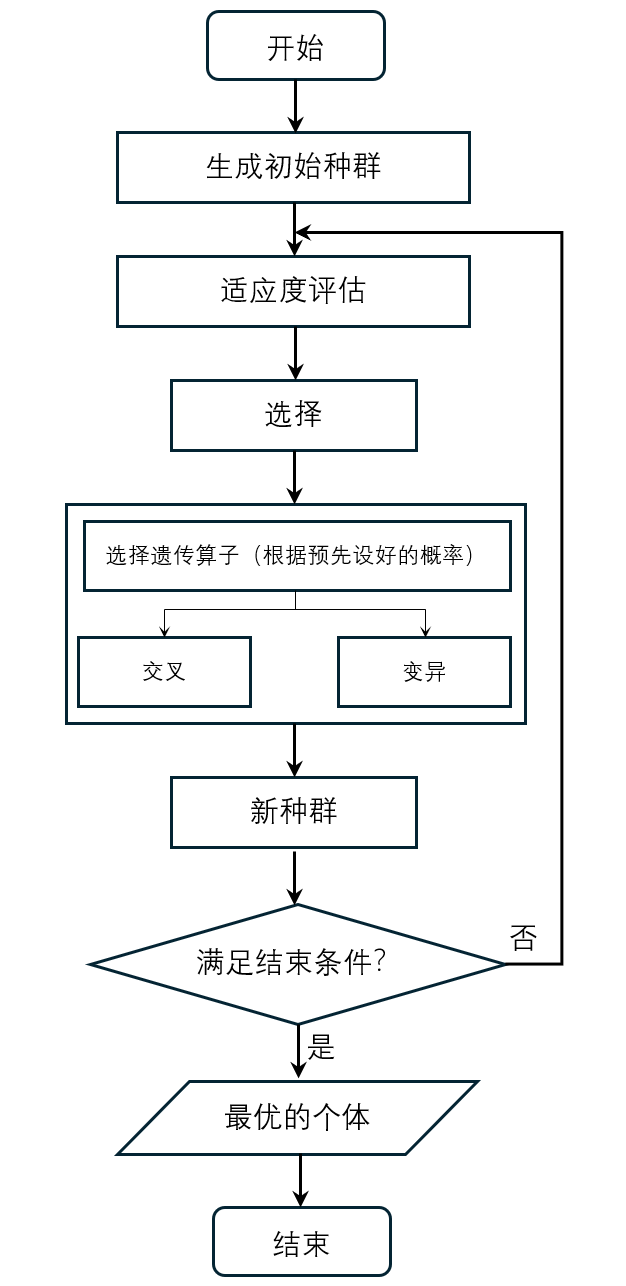
\includegraphics[width=5cm]{GA流程图.png}
        \subcaption{GA 与 GP流程图}
    \end{minipage}
    \begin{minipage}[t]{.5\textwidth}
        \centering
        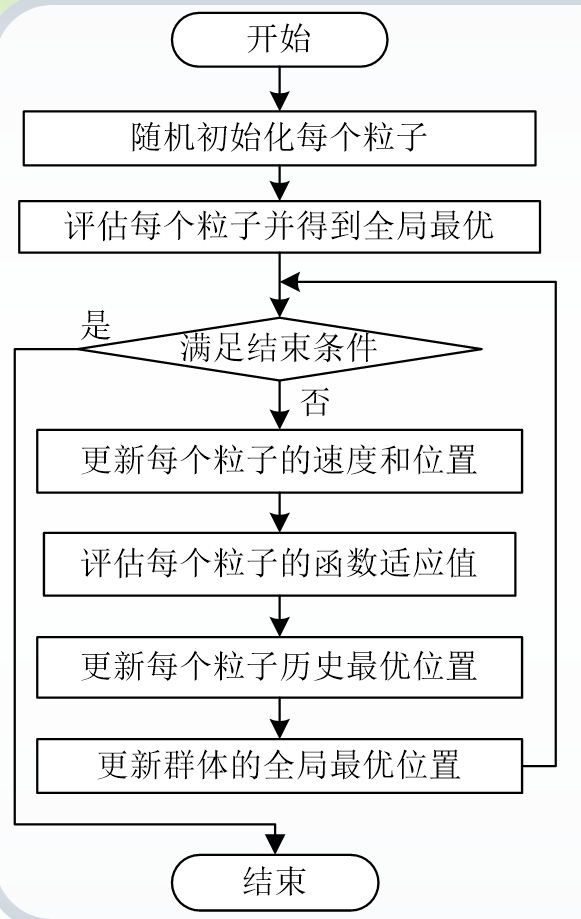
\includegraphics[width=5cm]{PSO流程图.png}
        \subcaption{PSO 流程图}
    \end{minipage} \\
    %\vspace{2em}
    \begin{minipage}[t]{\textwidth}
        \centering
        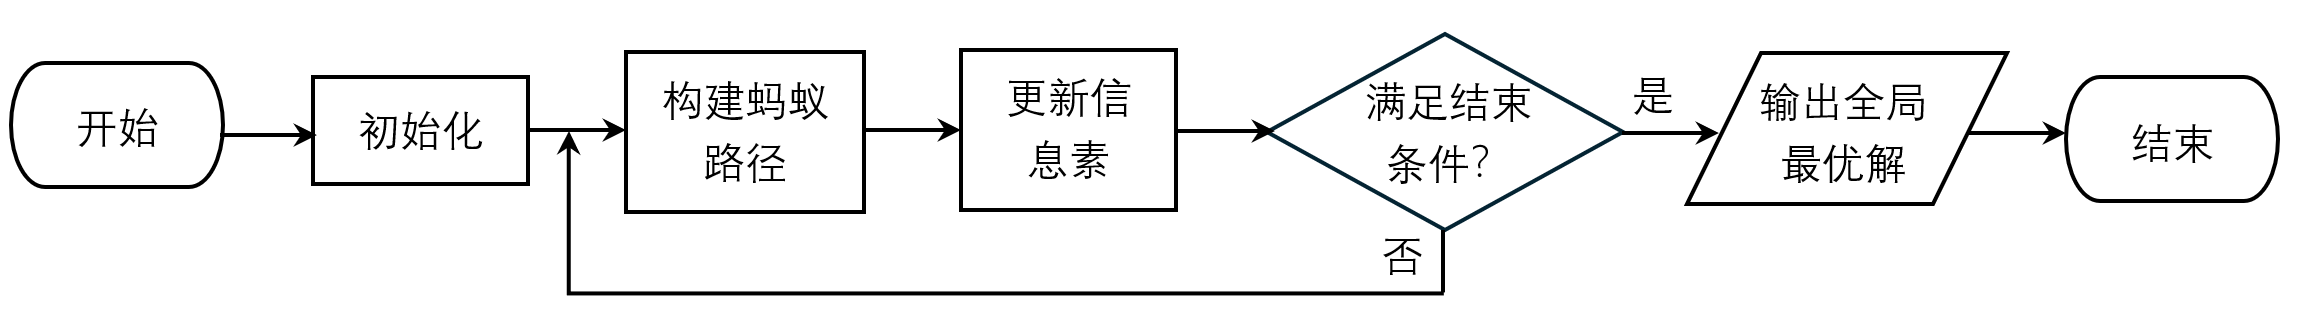
\includegraphics[width=\textwidth]{ACO流程图.png}
        \subcaption{ACO 流程图}
    \end{minipage}
  \caption{遗传算法(GA)、遗传编程(GP)、粒子群优化算法(PSO)、蚁群优化算法(ACO)流程图}\label{fig:GA,GP,PSO}
\end{figure}

编码与解码,基因型与表现型。编码有二进制编码、实数编码等方式,用于对染色体进行操作。

在 GA 中,个体通常为染色体。

\begin{process}{GA 简要流程}
\begin{enumerate}[itemsep=0pt,parsep=0pt]
  \item 初始化种群,个体编码。
  \item 评估适应度:$Fit=f(x)$ (最大化问题)或 $Fit=\dfrac{1}{f(x)}$(最小化问题)。可能需要尺度变换。
  \item 选择:轮盘赌法、锦标赛法。综合考虑精英策略。
  \item 交叉:一点交叉、两点交叉。
  \item 变异:单点变异、多点变异。
  \item 如果达到终止条件则终止,否则转第 2 步继续迭代。
\end{enumerate}
\end{process}


GA 的特点:数学要求不高,搜索效率高,易于并行化。

\subsection{GP「$\stackrel{\text{genetic programming}}{\text{\makebox[2.5cm][s]{遗传编程}}}$」}
在 GP 中,个体通常为种群树、问题的解等。

\begin{itemize}[itemsep=0pt,parsep=0pt]
  \item 终端集:叶节点,代表每个 GP 个体的输入。
  \item 功能集:非叶节点,代表终端数据间的运算。
  \item 此外,需考虑充分性和闭包,功能集的函数应完备(有加必有减),除法受除 0 保护等。
\end{itemize}

\begin{process}{GP 简要流程}
\begin{enumerate}[itemsep=0pt,parsep=0pt]
  \item 种群初始化:Full 法、Grow 法、Ramped half-and-half 法(一般取最后一种居多);
  \item 评估适应度:一般为分类成功率等;
  \item 选择:轮盘赌法、锦标赛法,综合考虑精英策略;
  \item 子树交叉:随机选择两个个体的子树互换;
  \item 子树变异:随机选择一个个体的子树,替换为随机生成的另一子树;
  \item 如果达到终止条件则终止,否则转第 2 步继续迭代。
\end{enumerate}
GP 的流程与 GA 一致,算法是共通的。
\end{process}

GP 的应用:分类,演化出最优的分类器个体。

GP 的缺点:训练时间较长。对时间有要求的不建议用 GP。\textcolor{cyan}{(数据规模:$\mathrm{PSO < GA < GP}$)}

代价敏感学习:对分类结果不平衡的一种特殊情境。可以将代价敏感规则结合 GA,GP,PSO,ACO 等设计算法。

相关问题:TSP「$\stackrel{\text{traveling salesman problem}}{\text{\makebox[3cm][s]{旅行商问题}}}$」。

\section{PSO「$\stackrel{\text{particle swarm optimization}}{\text{\makebox[5cm][s]{粒子群优化算法}}}$」}
PSO 是一种模仿鸟类觅食的算法,加入群体协作对个体认知的影响。PSO 的流程图如图 \ref{fig:GA,GP,PSO} 所示(见上页)。

PSO 和 GA 共通之处:种群需要初始化、个体需要编码、适应度需要评估,都是通过多轮迭代选出最优个体或者全局最优位置。

PSO 的速度决定式分三部分组成:
\begin{enumerate}[itemsep=0pt,parsep=0pt]
  \item 惯性权重 $\omega$:控制前一速度对当前速度的惯性影响;
  \item 个体加速系数 $c_1$:控制粒子 $i$ 向自身极值 $pBest_i$ 推进的加速权值;
  \item 群体加速系数 $c_2$:控制例子向全局极值 $gBest$ 推进的加速权值。
\end{enumerate}
没有惯性权重,则粒子的速度失去记忆性;没有个体加速系数,则粒子没有认知能力,完全「随大流」;没有群体加速系数,则粒子之间不存在交互,完全「各干各的」。

\begin{process}{PSO 简要流程}
\begin{enumerate}[itemsep=0pt,parsep=0pt]
  \item 粒子初始化,评估每个 $pBest_i$ 并得到全局最优 $gBest$。
  \item 更新粒子的速度和位置。
  \item 评估粒子的适应度。
  \item 更新每个 $pBest_i$ 和全局最优 $gBest$。
  \item 若满足结束条件则结束,否则转步骤 2 迭代。
\end{enumerate}
\end{process}

典型拓扑结构:星型结构、环型结构、齿型结构、冯诺依曼结构。

\begin{figure}[htb]
  \centering
  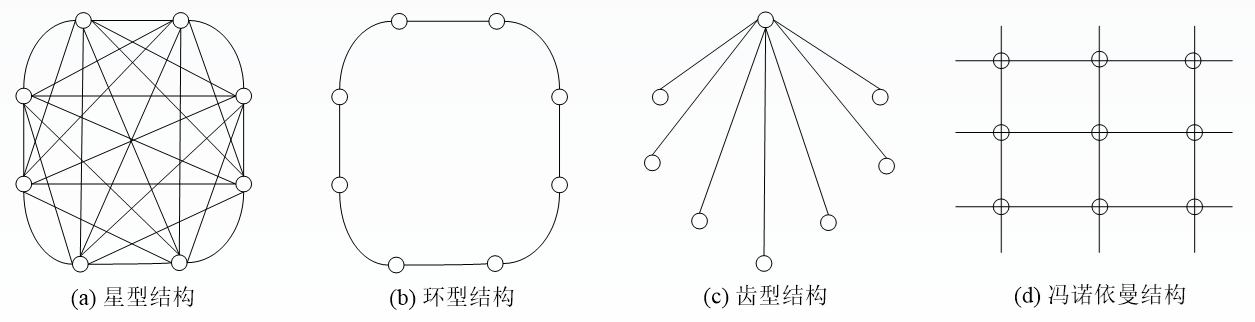
\includegraphics[width=\textwidth]{拓扑结构.png}
  \caption{典型拓扑结构}\label{fig:topo-structure}
\end{figure}

全局 PSO 和局部 PSO 的区别:
\begin{itemize}[itemsep=0pt,parsep=0pt]
  \item 全局 PSO (GPSO)收敛更快,但容易陷入局部最优。
  \item 局部 PSO (LPSO)多样性更高。
  \item 邻域较小,推荐局部 PSO;
  \item 邻域较大,推荐全局 PSO。
\end{itemize}

应用:基于粗糙集的粒子群和遗传算法综合算法(PSO-GA-RS):对于 $p$ 的数据用 PSO 处理,剩下 $1-p$ 的数据用 GA 处理。


\section{ACO「$\stackrel{\text{ant colony optimization}}{\text{\makebox[4cm][s]{蚁群优化算法}}}$」}
ACO 是一种模仿蚂蚁觅食的算法,通过信息素来寻找最优解。蚂蚁在寻找食物的过程中往往是随机选择路径的,但它们能感知当前地面上的信息素浓度,并倾向于往信息素浓度高的方向行进。

ACO 有两个基本要素:路径构建、信息素更新。

\begin{process}{ACO 简要流程}
\begin{enumerate}[itemsep=0pt,parsep=0pt]
  \item 初始化——设置蚂蚁数量、信息素权重、距离权重、蒸发率、最大迭代轮数等。
  \item 构建蚂蚁路径——将每只蚂蚁随机放至出发点,计算蚂蚁前往各结点的概率,用轮盘赌法决定要访问的下一结点。重复这一步直至蚂蚁路径构建完成。
  \item 更新信息素——根据路径更新信息素,并记录最优解。
  \item 判断结束——如果达到结束条件则结束算法,输出最优解;否则转第 2 步迭代计算。
\end{enumerate}
\end{process}

改进版本:精华蚂蚁系统、基于排列的蚂蚁系统、蚁群系统等。

\section{搜索求解策略}
按搜索方向分类:
\begin{itemize}[itemsep=0pt,parsep=0pt]
  \item 正向搜索——数据驱动;
  \item 逆向搜索——目的驱动;
  \item 双向搜索。
\end{itemize}

按搜索方式分类:盲目搜索、启发式搜索。

\subsection{状态空间表示}

在状态空间中,状态为结点,操作为边。
\begin{itemize}[itemsep=0pt,parsep=0pt]
  \item 状态:$Q = [q_1, q_2, \dots, q_n]^{\mathrm{T}}$
  \item 操作:$F = \{f_1, f_2, \dots, f_m\}$ (也用 $O$ 表示)
  \item 状态空间:$(S,O,S_0,G)$——(状态集,操作集,初始状态集,目标状态集)
  \item 求解路径:$S_0$ 到 $G$ 的路径。
  \item 可行解:由 $S_0$ 迁移到 $G$ 的那些边:$O_1,O_2,\dots,O_k$。
\end{itemize}
\textcolor{cyan}{(其中 $n,m,k$ 为自然数)}

\subsection{盲目搜索策略:DFS、BFS 算法}
一般的回溯思想:
\begin{itemize}[itemsep=0pt,parsep=0pt]
  \item PS 表——当前路径的状态
  \item NPS 表——未处理的新路径状态
  \item NSS 表——无解状态
  \item open 表即为 NPS 表(未搜索的状态)
  \item closed 表为 $\mathrm{PS \cup NSS}$ 表(已搜索的状态)。
\end{itemize}

宽度优先搜索(BFS)的次序是,先搜索第 1 层的结点,再搜索第 2 层,再搜索第 3 层……以此类推。(例:积木问题)

深度优先搜索(DFS)的次序是,保证每个结点的子状态比兄弟状态更先被搜索。(例:卒穿阵问题)

\subsection{启发式搜索策略:A、A* 算法}
相关概念:

\begin{itemize}[itemsep=0pt,parsep=0pt]
  \item 启发式信息:可以用于简化搜索过程的信息。
  \item 启发式策略:利用与问题有关的启发信息进行搜索。\textcolor{cyan}{(注:回忆第 3 章,有一种推理方式叫启发式推理。)}
  \item 估价函数:$f(n) = g(n)+h(n)$,从初始结点经过 $n$ 结点到目的结点的最小代价估计值。
  \item A 算法:对于下一结点,优先选择估价 $f(n)$ 较小的结点进行扩展。
  \item A* 算法:A 算法的最优形式。
\end{itemize}

例子:八数码问题。使用的 A 算法的估价函数是 $f(n) = d(n) + w(n)$,其中 $d(n)$ 为搜索树深度(根为0),$w(n)$ 为不在最终位置的数字个数。

\section{机器学习}
\subsection{机器学习概述}
\noindent\Emph{机器学习的分类}:
\begin{itemize}[itemsep=0pt,parsep=0pt]
  \item 监督学习——数据带标签,一般为回归、分类等任务
  \item 无监督学习——数据无标签,一般为聚类等任务
  \item 强化学习——序列数据决策学习,一般通过与环境交互来学习
\end{itemize}

\noindent 典型的机器学习过程(以分类任务为例):训练数据 $\to$ 训练学习算法 $\to$ 得到模型 $\to$ 输出新样本的分类结果

\noindent 「泛化误差」与「经验误差」:
\begin{itemize}[itemsep=0pt,parsep=0pt]
  \item 泛化误差——在未来样本上的误差,自然是越小越好;
  \item 经验误差——在训练集上的误差,但并不是越小越好(过小反而易导致过拟合)。
\end{itemize}

\noindent\Emph{「过拟合」}与「欠拟合」:
\begin{itemize}[itemsep=0pt,parsep=0pt]
  \item 过拟合——模型学习了一些无关紧要的特征,甚至包括噪声;
  \item 欠拟合——模型学习不到位,遗漏了重要特征;
  \item 通常训练样本少、维度高,更有可能出现过拟合。
\end{itemize}

\noindent 典型的评估方法(获取测试集):
\begin{itemize}[itemsep=0pt,parsep=0pt]
    \item 留出法——将训练集与测试集分开。
    \begin{itemize}[itemsep=0pt,parsep=0pt]
      \item 这种方法需要假设数据是平衡的;
      \item 可通过分层采样保持数据一致性;
      \item 可多次重复划分,且测试集所占比例一般为 $\frac15\sim\frac13$ 为宜。
    \end{itemize}
    \item $k$ 折交叉验证法——将原始数据集均分为 $k$ 份,进行 $k$ 轮,每轮取一份作测试集,交叉变换,取 $k$ 轮测试结果的平均值作为最终结果。
\end{itemize}

\noindent 典型的性能度量指标:错误率、精度、查准率、查全率、F-score、$F_1$、$F_\beta$ 等。

\noindent 对于分类问题,还可以用真阳性率关于假阳性率的图像(ROC 曲线)作为分类图,其曲线下方面积 AUC 常用作分类指标。

\subsection{$k$ 近邻(KNN)}
对于测试样本,找到离其「最近」的 $k$ 个样本,用投票法或平均法获知分类或预测结果。当 $k$ 取不同值时,分类结果会有不同。

特点:\Emph{没有训练过程},也称为「懒惰学习」、「急切学习」。这种方法的测试过程比较耗时,需要大量计算距离。

「距离」的定义也是重要的一环:计算维度更高的数据的「距离」会更慢,而且需要统一量纲。

\subsection{决策树算法}
决策树是基于树形结构决策的算法,具体包含 ID3、C4.5、CART 等算法。
\begin{itemize}[itemsep=0pt,parsep=0pt]
  \item 叶结点——分类结果
  \item 非叶结点——属性
  \item 边——属性的值
\end{itemize}

\begin{process}{决策树算法简要流程}
对决策树的每一层,遵循以下流程:
\begin{enumerate}[itemsep=0pt,parsep=0pt]
  \item 对于每一种属性(如色泽、纹理),计算其每一个子集的信息熵;
  \item 计算这种属性的信息增益;
  \item 选取信息增益最大的属性作为当前层的划分属性;
  \item 对子结点递归地操作,直到所有属性划分完成,得到决策树。
\end{enumerate}
\end{process}

相关指标:信息熵、信息增益、增益率、基尼指数等。

\subsection{SVM「$\stackrel{\text{support vector machines}}{\text{\makebox[3cm][s]{支持向量机}}}$」}
SVM 的目标:找到超平面,使得它能够尽可能正确地区分两类数据,并使两类数据点距离该超平面最远。

SVM 是一个\Emph{强分类器}。

SVM 有以下两种「法宝」:
\begin{itemize}
  \item 核函数——用于将线性不可分的数据点映射到更高维度
  \item 软间隔——允许少量数据点不满足约束
\end{itemize}

\subsection{集成学习}
集成学习是指,将多个学习器(弱分类器)结合在一起,提升性能(得到强分类器)。集成个体之间应满足「好而不同」原则。

集成学习器有以下组织方式:
\begin{enumerate}[itemsep=0pt,parsep=0pt]
  \item \Emph{Boosting}——串行生成,个体之间依赖性强,每次调整训练数据的样本分布;
  \item \Emph{Bagging}——并行生成,个体之间依赖性弱,采用自助采样法;
  \item 随机森林——是 Bagging 的一个变种,强调采样与属性选择的随机性。
\end{enumerate}

集成学习器有以下结合策略:
\begin{enumerate}[itemsep=0pt,parsep=0pt]
    \item 平均法——简单、加权平均
    \item 投票法——绝对多数、相对多数、加权投票法
\end{enumerate}
此外,加权平均法未必优于简单平均法。

\subsection{$k$-means 聚类}
聚类目标:将数据集样本划分为若干个「簇」。

聚类既可用作单独过程,也可用作其他任务的前置过程。

\begin{process}{$k$-means 聚类简要流程}
\begin{enumerate}[itemsep=0pt,parsep=0pt]
  \item 初始化每个簇的均值向量;
  \item 更新簇划分;
  \item 计算每个簇的均值向量;
  \item 如果当前均值向量均未更新,结束;否则转步骤 2 迭代计算。
\end{enumerate}
\end{process}

\section{人工神经网络}
\subsection{神经元与神经网络}
神经网络方法是一种隐式的知识表示方法。

神经元数学模型:从各输入端接收输入信号,求出加权和,用激励函数转换输出。

几个相关函数:
\begin{table}[htb]
  \centering
  \begin{tabular}{cccc}
  \toprule
    ReLU 函数 & 硬极限函数 & 对称硬极限函数 \\
  \midrule
    $y = \begin{cases} 0, \ x<0 \\ x,\ x\geqslant 0\end{cases}$ &
    $y = \begin{cases} 0, \ x<0 \\ 1,\ x\geqslant 0\end{cases}$ &
    $y = \begin{cases} -1, \ & x<0 \\ 1,\ & x\geqslant 0\end{cases}$ \\
  \bottomrule
  \end{tabular}
  \caption{神经网络领域的常用函数}\label{fig:func}
\end{table}

\begin{itemize}[itemsep=0pt,parsep=0pt]
  \item 神经网络的结构:前馈型、反馈型
  \item 神经网络的工作方式:同步方式、异步方式
\end{itemize}

\subsection{BP 神经网络与 BP 算法}
BP 神经网络是典型的\Emph{前馈型}结构。作为对比:Hopfield 神经网络是典型的「反馈型」。

求解 BP 神经网络权重的原理是「梯度下降算法」。

BP 算法也称为「$\stackrel{\text{back propagation}}{\text{误差反向传播算法}}$」,是对神经网络进行更新的一种算法。

\begin{process}{BP 算法的简要流程}
\begin{enumerate}[itemsep=0pt,parsep=0pt]
  \item 初始化——对所有连接权和阈值赋值为随机任意小值 $w_{ij}(0),\ \theta_i(0)$;
  \item 输入——从 $N$ 组样本中选取一组样本输入到 BP 神经网络中;
  \item 计算输出——计算各层结点的输出 $y_i$;
  \item 计算误差——计算网络实际输出与期望输出的误差 $e_i$;
  \item 反向传播——从输出层计算到第一个隐层,依次修改连接权值;
  \item 判断——如果 $N$ 组样本的误差均达到要求,结束;否则取另一组样本转步骤 2 计算。
\end{enumerate}
\end{process}

BP 神经网络的优缺点:
\begin{description}[itemsep=0pt,parsep=0pt]
  \item[优点] 逼近特性强,泛化能力强,容错性高;
  \item[缺点] 收敛速度慢,局部极值,难以确定隐层信息(解释性较差)。
\end{description}

\subsection{深度学习、卷积神经网络}
深度学习的流程是:获取数据—数据清洗—特征提取—特征选择—推理预测识别。其中特征提取、特征选择两个步骤又合称为「特征表达」,这是识别成功的关键。

深度学习是以端到端的方式逐层抽象,逐层学习的方式。

CNN「$\stackrel{\text{convolutional neural networks}}{\text{\makebox[3cm][s]{卷积神经网络}}}$」是一个多层的神经网络,每一个卷积层都跟着一个池化层。
\begin{description}[itemsep=0pt,parsep=0pt]
  \item[卷积层] 也称 C (convolutional)层,用于特征提取;
  \item[池化层] 也称 S (subsampling)层,用于特征选择。
\end{description}

对于卷积层,求卷积的过程应当掌握。对图像用卷积核进行卷积运算,实际上是滤波的过程,可以得到显著的边缘特征。

对于池化层,常用的池化操作有最大池化、平均池化等。池化层在语义上把相似的特征合并,降低了空间分辨率。

减少参数数量的方法:局部连接、权值共享。

\subsection{生成对抗网络}
GAN「$\stackrel{\text{generative adversarial networks}}{\text{\makebox[3cm][s]{生成对抗网络}}}$」有两个角色:生成器和判别器,如同假币制造机与验钞机一般。

生成器用来生成数据,判别器用来判断数据的真假。通过不断训练,尽可能让生成器生成更真实的数据,直至判别器无法再判别数据的真实性。

GAN 有两个相互交替的学习阶段:
\begin{itemize}[itemsep=0pt,parsep=0pt]
  \item 固定生成网络,训练判别网络;
  \item 训练生成网络,固定判别网络。
\end{itemize}

\backgroundsetup{contents=
\includegraphics{下半示例.png}, center, scale=1, angle=0, opacity=1}
\BgThispage

典型应用:图像处理。

GAN 的训练结果随机性较大,具有强烈的不稳定性,难以收敛。

\end{document} 